\chapter{Flexion simple (cisaillante)}
\section{En route vers l'incohérence}
	\subsection{Méthode cinématique}
	On postule le même	champ de déplacement que pour la flexion pure mais
	on ne postulera \textbf{pas} la conservation des normales (hypothèse 
	de Bernoulli)	
	\begin{equation}
	u=z\beta_x(x),\qquad v=0,\qquad w=w_0(x).
	\end{equation}
	
	\subsection{Déplacements – Déformations – Contraintes}
		\subsubsection{Déformation angulaire}
		Ici la section va tourner, l'axe va également tourner mais leurs 
		angles de rotation ne seront plus identiques (ce qui était le cas 
		avec Bernoulli). En effet, l'hypothèse de Bernoulli est incompatible 
		avec un effort tranchant non-nul, il faut l'abandonner.\\
		
		On \textbf{ne} suppose donc \textbf{pas} que les normales à la 
		section droite restent normales après déformation : il y a variation 
		d'angle $\rightarrow \gamma_{xz} \neq 0$.
		On \textbf{remplace} l'hypothèse de Bernoulli par : \textit{dans la 
		configuration déformée, les sections droites initialement planes 
		restent planes (mais ne restent pas perpendiculaires à l'axe déformé).}
		
		\subsubsection{Flexion autour de $z$}
		Étudions la flexion autour de $z$ pour le déplacement $u=y\alpha_x(x); 
		v=v_0(x);w=0$. Plaçons nous à l'intérieur d'une section. Dans une 
		section $\alpha_x$ est le même en tout point de la section : il ne 
		dépend donc pas de $y$ et $z$. Comme on considère $v_0(x)$, tous les 
		points de la section subissent le même déplacement : il ne dépend pas 
		non plus de $y$ et $z$. Forcément, $\gamma_{xy}$ est également 
		constant dans une section, impliquant que $\tau_{xy}$ l'est aussi.
		\begin{equation}
		\gamma_{xy} = \alpha_x + \dfrac{\partial v_0}{\partial x}\qquad
		\Longrightarrow\qquad \tau_{xy} = G\gamma_{xy}
		\end{equation}
		Mais est-ce possible ? Nous savons que $\tau_{xy}$ est nul en surface 
		car il n'y a pas de force de freinage (de même en dessous). Or, 
		$\tau_{xy}$ doit être constant (de 0 à 0) mais avec une résultante 
		non nulle (nous venons de le démontrer) : le résultat est incohérent 
		et n'est évidemment pas possible.  Mathématiquement, cette incohérence 
		s'exprime :
		\begin{equation}
		\tau_{xy} =\ cste\quad \Leftrightarrow \tau_{xy}=0\qquad \Longrightarrow 
		T_y = \int_A \tau_{xy}\ dA = 0\quad \Longrightarrow \text{Pas d'effort 
		tranchant}
		\end{equation}


\section{Jourawski}
La RDM étant une approximation de l'élasticité, il va falloir procéder 
autrement, via une solution approchée.	
	
	\subsection{Un peu d'histoire}		
	\begin{wrapfigure}[6]{r}{9cm}
	\vspace{-7mm}
	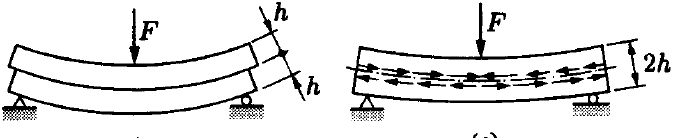
\includegraphics[scale=0.4]{ch5/image1.png}
	\captionof{figure}{ }
	\end{wrapfigure}
	Jourawski devait employer des poutres en bois pour la construction d'ouvrages 
	d'art d'une ligne de chemin et cherchait à augmenter la résistance et la 
	rigidité de ces poutres. Il a remarqué que si deux poutres étaient mise 
	l'une au dessus de l'autre et qu'elle ne pouvaient glisser l'une sur l'autre, 
	le moment d'inertie et le module de flexion de la structure seraient 
	respectivement quatre et deux fois plus élevé que dans le cas ou les poutres 
	peuvent glisser librement.
	Grâce à quoi ? A la présence de contraintes tangentielles (\textit{contraintes 
	rasantes}) qui obligent les fibres des faces communs à garder la même 
	longueur\footnote{Sinon les fibres inférieures de la poutre du haut s'allongent 
	et les fibres supérieures de la poutre du dessous se raccourcissent.}.\\
	Comment faire apparaître ces contraintes tangentielles? En plaçant des cales 
	empêchant le glissement entre les poutres.
	
	\subsection{Principe du calcul des contraintes tangentielles}
	\begin{wrapfigure}[7]{l}{7cm}
	\vspace{-7mm}
	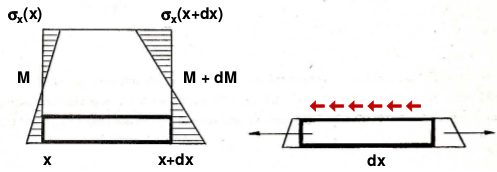
\includegraphics[scale=0.4]{ch5/image2.png}
	\captionof{figure}{ }
	\end{wrapfigure}
	Savoir qu'il en faut c'est bien, pouvoir les calculer c'est mieux! Considérons 
	un tronçon de poutre compris entre $x$ et $x+dx$ soumis aux moments fléchissants 
	$M$ et $M+dM = M(x+dx)$. Les répartitions des contraintes normales suivent la 
	même logique $\sigma_x(x)$ et $\sigma_x(x+dx)$. Isolons une partie intérieure 
	de ce tronçon par une coupe horizontale.\\	
	On remarque qu'il faut ajouter des contraintes tangentielles pour équilibrer 
	les forces introduites. Autrement dit, comme les contraintes ne s'équilibrent 
	pas, l'équilibre axial doit être assuré par l'effort rasant le long de la 
	coupe horizontale.
	
	\subsection{Équilibre de translation axial}
	Soit une partie cylindrique d'un tronçon de poutre $dx$. On considère qu'il 
	n'y a pas de force de volume. De plus, nous savons que
	\begin{equation}
	\oint T_x^{(n)}\ dS = 0
	\end{equation}
	Écrivons l'équilibre de translation axial
	\begin{equation}
	\int_\Sigma T_x^{(-x)}\ dS + \int_{\Sigma'} T_x^{(x)}\ dS + \int_{coupe} T_x^{(n)}\ 
	dS + \underbrace{\int_{S_{lat}}T_x^{(n)}\ dS}_{=0} = 0
	\end{equation}\newpage	ccc
	Le dernier terme est nul car il n'y a pas de force tangentielle en surface. 
	En considérant une poutre prismatique\footnote{Pq?}
	\begin{eqnarray}
	\int_\Sigma [\sigma_x(x+dx)-\sigma_x(x)]\ dS + \int_{coupe} \tau_{nx}\ dLdx = 0\\
	\int_\Sigma \dfrac{\partial \sigma_x}{\partial x}\ dxdS + \underbrace{\int_{coupe} 
	\tau_{nx}\ 	dLdx = 0}_{\text{Effort rasant}}
	\end{eqnarray}
	Après division par $dx$ :
	\begin{equation}
	\int_\Sigma \dfrac{\partial \sigma_x}{\partial x}\ dS + \int_{AB}\tau_{nx}\ dL=0
	\end{equation}
	La répartition de la contrainte 
	axiale $\sigma_x$ dans une section est donné par\footnote{Hypothèse des sections 
	planes restant planes.} :$\sigma_x = \dfrac{M}{I}y$.
	Avec la relation $T\leftrightarrow M$, on trouve 
	\begin{equation}
	\dfrac{dM}{dx}= T\qquad\Longrightarrow\qquad \dfrac{\partial\sigma_x}{\partial x}
	=\dfrac{T}{I}y
	\end{equation}
	Avec $\int_\Sigma \dfrac{\partial \sigma_x}{\partial x}\ dS + \int_{AB}\tau_{nx}\ 
	dL=0$ on trouve
	\begin{equation}
	\int_{AB}\tau_{nx}\ dL = -\dfrac{T}{I}\int_\Sigma y\ dS\qquad\text{ ou }\qquad 
	\int_{AB} \tau_{nx}\ dL = -\dfrac{T}{I}S(\Sigma)
	\end{equation}
	où $S(\Sigma) = \int_\Sigma y\ dS$ est le moment statique de la surface $\Sigma$ 
	par rapport à l'axe neutre.\\
	\danger\  $I$ est le moment d'inertie par rapport à l'axe neutre, de \textbf{toute} 
	section transversale.
	
	\subsection{Contrainte tangentielle moyenne}
	\begin{wrapfigure}[7]{r}{2cm}
	\vspace{-7mm}
	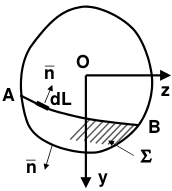
\includegraphics[scale=0.4]{ch5/image4.png}
	\captionof{figure}{ }
	\end{wrapfigure}
	On la définit (ci-contre, le plan de coupe de la précédente figure)
	\begin{equation}
	\overline{\tau}_{nx} = \dfrac{1}{L_{AB}}\int_{AB}\tau_{nx}\ dL
	\end{equation}
	Or comme $\int_{AB} \tau_{nx}\ dL = -\dfrac{T}{I}S(\Sigma)$, on obtient 
	\begin{equation}
	\overline{\tau}_{nx} = -\dfrac{T}{I}\dfrac{S(\Sigma)}{L_{AB}}
	\end{equation}
	
	
	\subsection{Formule de Jourawski}
	\begin{wrapfigure}[3]{l}{3cm}
	\vspace{-7mm}
	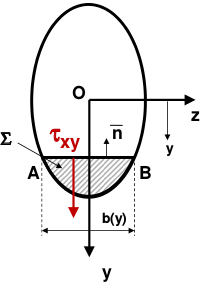
\includegraphics[scale=0.4]{ch5/image5.png}
	\captionof{figure}{ }
	\end{wrapfigure}
	Si l'arc $AB$ est une droite parallèle à l'axe $z$, on peut repartir de 
	$\overline{\tau}_{nx} = -\dfrac{T}{I}\dfrac{S(\Sigma)}{L_{AB}}$ en sachant 
	que $\overline{\tau}_{nx} = -\overline{\tau}_{xy}$, pour finalement obtenir 
	\begin{equation}
	\overline{\tau}_{xy} = \dfrac{T}{I}\dfrac{S(\Sigma)}{b}
	\end{equation}
		
		\subsubsection{Réciprocité des contraintes tangentielles}
		Pour faire bref $\tau_{nx} = \tau_{xn}$ et $\tau_{yx}=\tau_{xy}$. On 
		trouve alors :
		\begin{equation}
		\begin{array}{lll}
		\overline{\tau}_{xy} &= \dfrac{T}{I}\dfrac{S(\Sigma)}{b}; & \text{Contrainte 
		tangentielle moyenne}\\
		(b\overline{\tau}_{xy}) &= \dfrac{T}{I}S(\Sigma); & \text{Effort rasant}
		\end{array}
		\end{equation}		
		\textsc{Exemple :} slide 22.
	
	
\section{Déformation due à l'effort tranchant}
C'est le cas ou l'hypothèse "\textit{les sections planes restent planes}" n'est plus 
satisfaite : $\tau_{xy}$ pas constant $\rightarrow \gamma_{xy}$ pas constant $\Rightarrow 
$ les sections gauchissent $\Rightarrow$ théorie de Timoshenko.
	
	
